\documentclass[11pt]{article}
\usepackage[utf8]{inputenc}
\usepackage{amsmath}
\usepackage{multicol}
\usepackage{geometry}
\usepackage{tikz}
\usetikzlibrary{arrows.meta}
\usepackage{enumitem}
\usepackage{xcolor}
\usepackage{titlesec}

\geometry{a4paper, left=1.5cm, right=1.5cm, top=1.5cm, bottom=1.5cm}

% Definir as cores das seções
\titleformat{\section}
  {\normalfont\Large\bfseries\color{blue}}
  {\thesection}
  {1em}
  {}

\renewcommand{\thesubsection}{\textcolor{red}{\arabic{section}.\arabic{subsection}}}
\titleformat{\subsection}{\color{red}\normalfont\bfseries}{\thesubsection}{1em}{}

\title{\textcolor{blue}{Progressão Parcial referente à série do 1º ano do Ensino Médio}}
\author{Professor: Jefferson}
\date{}

\begin{document}

\maketitle

\begin{center}
\large{Nome: \underline{\hspace{8cm}} \quad Série-Turma: \underline{\hspace{3cm}}}
\end{center}

\setlength{\columnsep}{20pt}
\setlength{\columnseprule}{0.4pt}

\begin{multicols}{2}

\section*{Assunto:}
\begin{itemize}
    \item Plano cartesiano
    \item Funçao do 1º Grau
    \item Função do 2º grau
    \item Equação do 1º Grau
    \item Equação do 2º Grau
\end{itemize}

\section*{1. O Plano Cartesiano}
O plano cartesiano é um sistema de coordenadas que permite visualizar graficamente a relação entre duas variáveis. É formado por duas retas numéricas perpendiculares:
\begin{itemize}
    \item O eixo horizontal é chamado de \textbf{eixo x} (abscissa).
    \item O eixo vertical é chamado de \textbf{eixo y} (ordenada).
\end{itemize}
A interseção deles é a origem \(O = (0, 0)\). Qualquer ponto \(P\) neste plano é representado por um par ordenado \((x, y)\).

\begin{center}
\begin{tikzpicture}[scale=0.7]
\draw[->] (-3, 0) -- (3, 0) node[right]{\(x\)};
\draw[->] (0, -2) -- (0, 3) node[above]{\(y\)};
\draw[fill] (2, 1) circle (2pt) node[above right]{\(P(2, 1)\)};
\draw[dashed] (2, 0) -- (2, 1);
\draw[dashed] (0, 1) -- (2, 1);
\end{tikzpicture}
\end{center}

\subsection*{Atividade Resolvida}
\textbf{Questão:} Marque os seguintes pontos no plano cartesiano: \(A(1, 2)\), \(B(-2, 3)\), \(C(0, -1)\), \(D(-1, -2)\).

\textbf{\textcolor{blue}{Resolução:} }
\begin{itemize}
    \item Para \(A(1, 2)\): anda-se 1 unidade para a direita no eixo x e 2 unidades para cima no eixo y.
    \item Para \(B(-2, 3)\): anda-se 2 unidades para a esquerda no eixo x e 3 unidades para cima no eixo y.
    \item Para \(C(0, -1)\): permanece na origem no eixo x e anda-se 1 unidade para baixo no eixo y.
    \item Para \(D(-1, -2)\): anda-se 1 unidade para a esquerda no eixo x e 2 unidades para baixo no eixo y.
\end{itemize}

\begin{center}
\begin{tikzpicture}[scale=0.6]
\draw[->] (-3, 0) -- (3, 0) node[right]{\(x\)};
\draw[->] (0, -3) -- (0, 4) node[above]{\(y\)};
\filldraw (1, 2) circle (2pt) node[above right]{\(A\)};
\filldraw (-2, 3) circle (2pt) node[above left]{\(B\)};
\filldraw (0, -1) circle (2pt) node[below right]{\(C\)};
\filldraw (-1, -2) circle (2pt) node[below left]{\(D\)};
\end{tikzpicture}
\end{center}

\section*{2. Leitura de Gráficos do 1º Grau}
A leitura de gráficos é uma habilidade fundamental para interpretar relações entre grandezas. No gráfico de uma função do 1º grau, podemos identificar:
\begin{itemize}
    \item O coeficiente linear (ponto onde a reta corta o eixo y)
    \item A raiz da função (ponto onde a reta corta o eixo x)
    \item O crescimento ou decrescimento da função
\end{itemize}

\subsection*{Atividades de Leitura de Gráficos - 1º Grau}

\textbf{Questão 1:} Observe o gráfico da função \(f(x) = 2x - 4\) abaixo e responda:

\begin{center}
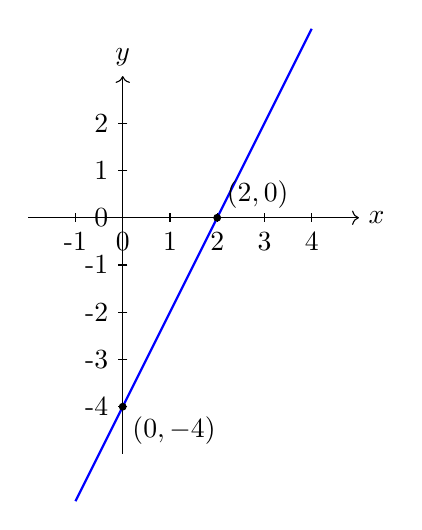
\begin{tikzpicture}[scale=0.6]
\draw[->] (-2, 0) -- (5, 0) node[right]{\(x\)};
\draw[->] (0, -5) -- (0, 3) node[above]{\(y\)};
\draw[domain=-1:4, smooth, variable=\x, blue, thick] plot ({\x}, {2*\x - 4});
\filldraw (0, -4) circle (2pt) node[below right]{\((0, -4)\)};
\filldraw (2, 0) circle (2pt) node[above right]{\((2, 0)\)};
\foreach \x in {-1,0,1,2,3,4}
    \draw (\x,0.1) -- (\x,-0.1) node[below] {\x};
\foreach \y in {-4,-3,-2,-1,0,1,2}
    \draw (0.1,\y) -- (-0.1,\y) node[left] {\y};
\end{tikzpicture}
\end{center}

a) Qual é o coeficiente linear da função? \\
\textbf{\textcolor{blue}{Resposta:}} O coeficiente linear é \(b = -4\), pois a reta corta o eixo y no ponto \((0, -4)\).

b) Qual é a raiz da função? \\
\textbf{\textcolor{blue}{Resposta:}} A raiz é \(x = 2\), pois é onde a reta corta o eixo x no ponto \((2, 0)\).

c) A função é crescente ou decrescente? Justifique. \\
\textbf{\textcolor{blue}{Resposta:}} A função é crescente, pois conforme \(x\) aumenta, o valor de \(y\) também aumenta (a reta sobe da esquerda para a direita).

\textbf{Questão 2:} Analise o gráfico da função \(f(x) = -x + 3\):

\begin{center}
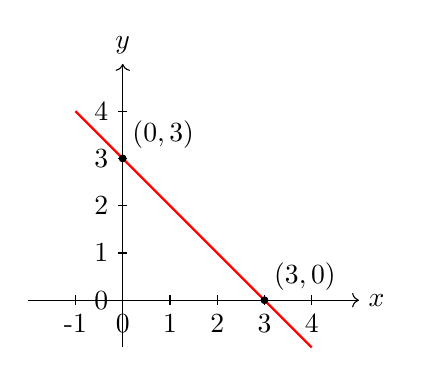
\begin{tikzpicture}[scale=0.6]
\draw[->] (-2, 0) -- (5, 0) node[right]{\(x\)};
\draw[->] (0, -1) -- (0, 5) node[above]{\(y\)};
\draw[domain=-1:4, smooth, variable=\x, red, thick] plot ({\x}, {-\x + 3});
\filldraw (0, 3) circle (2pt) node[above right]{\((0, 3)\)};
\filldraw (3, 0) circle (2pt) node[above right]{\((3, 0)\)};
\foreach \x in {-1,0,1,2,3,4}
    \draw (\x,0.1) -- (\x,-0.1) node[below] {\x};
\foreach \y in {0,1,2,3,4}
    \draw (0.1,\y) -- (-0.1,\y) node[left] {\y};
\end{tikzpicture}
\end{center}

a) Determine o valor de \(f(2)\) observando o gráfico. \\
\textbf{\textcolor{blue}{Resposta:}} Quando \(x = 2\), o valor de \(y\) é \(1\). Portanto, \(f(2) = 1\).

b) Para que valor de \(x\) temos \(f(x) = 2\)? \\
\textbf{\textcolor{blue}{Resposta:}} Quando \(y = 2\), o valor de \(x\) é \(1\). Portanto, \(f(1) = 2\).

c) Qual é a equação dessa reta? \\
\textbf{\textcolor{blue}{Resposta:}} A reta tem coeficiente linear \(b = 3\) e coeficiente angular \(a = -1\) (pois cai 1 unidade para cada aumento de 1 em x). Portanto, \(f(x) = -x + 3\).

\section*{3. Função do 1º Grau (Função Afim)}
Uma função do 1º grau estabelece uma relação onde a variável \(y\) depende de \(x\) de forma linear.

\subsection*{Definição}
Pode ser escrita na forma:
\[
f(x) = ax + b \quad \text{ou} \quad y = ax + b
\]
onde \(a\) e \(b\) são constantes reais, e \(a \neq 0\).

\subsection*{Gráfico no Plano Cartesiano}
O gráfico de uma função do 1º grau é sempre uma \textbf{reta}. Para desenhá-la, precisamos de pelo menos dois pontos.

\subsection*{Atividades Resolvidas}

\textbf{Questão 1:} Para a função \(f(x) = -3x + 4\), identifique \(a\) e \(b\) e classifique-a como crescente ou decrescente.

\textbf{\textcolor{blue}{Resolução:} }
\begin{itemize}
    \item Coeficiente angular: \(a = -3\)
    \item Coeficiente linear: \(b = 4\)
    \item Como \(a = -3 < 0\), a função é \textbf{decrescente}.
\end{itemize}

\textbf{Questão 2:} Construa o gráfico da função \(y = x + 2\) no plano cartesiano.

\textbf{\textcolor{blue}{Resolução:} }
Escolhendo dois valores para \(x\):
\begin{itemize}
    \item Para \(x = 0\): \(y = 0 + 2 = 2\) \(\rightarrow\) ponto \(A(0, 2)\)
    \item Para \(x = 2\): \(y = 2 + 2 = 4\) \(\rightarrow\) ponto \(B(2, 4)\)
\end{itemize}

\begin{center}
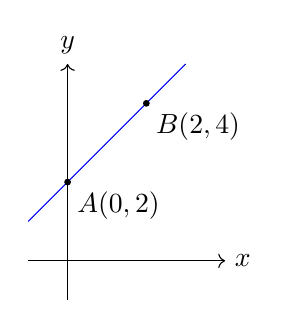
\begin{tikzpicture}[scale=0.5]
\draw[->] (-1, 0) -- (4, 0) node[right]{\(x\)};
\draw[->] (0, -1) -- (0, 5) node[above]{\(y\)};
\draw[domain=-1:3, smooth, variable=\x, blue] plot ({\x}, {\x + 2});
\filldraw (0, 2) circle (2pt) node[below right]{\(A(0, 2)\)};
\filldraw (2, 4) circle (2pt) node[below right]{\(B(2, 4)\)};
\end{tikzpicture}
\end{center}

\section*{4. Equação do 1º Grau}
Uma equação do 1º grau em uma variável é uma igualdade que pode ser reduzida à forma \(ax + b = 0\), com \(a \neq 0\). Resolvê-la significa encontrar o valor de \(x\) que satisfaz a igualdade.

\subsection*{Atividades Resolvidas}

\textbf{Questão 1:} Resolva as equações: \(2x - 7 = 3\) e \(-x + 4 = 10\).

\textbf{\textcolor{blue}{Resolução:} }
\[
2x - 7 = 3 \implies 2x = 3 + 7 \implies 2x = 10 \implies x = 5
\]
\[
-x + 4 = 10 \implies -x = 10 - 4 \implies -x = 6 \implies x = -6
\]

\textbf{Questão 2:} Encontre a raiz (zero) da função \(f(x) = 4x - 12\).

\textbf{\textcolor{blue}{Resolução:} }
A raiz é o valor de \(x\) que torna \(f(x) = 0\):
\[
4x - 12 = 0 \implies 4x = 12 \implies x = 3
\]
Portanto, a raiz da função é \(x = 3\). Geometricamente, este é o ponto onde a reta cruza o eixo x.

\section*{5. Leitura de Gráficos do 2º Grau}
No gráfico de uma função do 2º grau (parábola), podemos identificar:
\begin{itemize}
    \item A concavidade (para cima se \(a > 0\), para baixo se \(a < 0\))
    \item O vértice (ponto máximo ou mínimo)
    \item As raízes (pontos onde a parábola cruza o eixo x)
    \item O intercepto y (ponto onde a parábola cruza o eixo y)
\end{itemize}

\subsection*{Atividades de Leitura de Gráficos - 2º Grau}

\textbf{Questão 1:} Observe o gráfico da parábola abaixo e responda:

\begin{center}
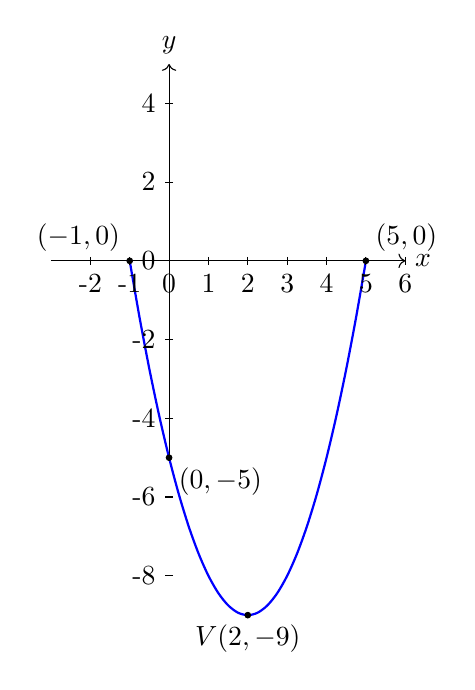
\begin{tikzpicture}[scale=0.5]
\draw[->] (-3, 0) -- (6, 0) node[right]{\(x\)};
\draw[->] (0, -5) -- (0, 5) node[above]{\(y\)};
\draw[domain=-1:5, smooth, variable=\x, blue, thick] plot ({\x}, {\x*\x - 4*\x - 5});
\filldraw (2, -9) circle (2pt) node[below]{\(V(2, -9)\)};
\filldraw (-1, 0) circle (2pt) node[above left]{\((-1, 0)\)};
\filldraw (5, 0) circle (2pt) node[above right]{\((5, 0)\)};
\filldraw (0, -5) circle (2pt) node[below right]{\((0, -5)\)};
\foreach \x in {-2,-1,0,1,2,3,4,5,6}
    \draw (\x,0.1) -- (\x,-0.1) node[below] {\x};
\foreach \y in {-8,-6,-4,-2,0,2,4}
    \draw (0.1,\y) -- (-0.1,\y) node[left] {\y};
\end{tikzpicture}
\end{center}

a) Qual é a concavidade da parábola? \\
\textbf{\textcolor{blue}{Resposta:}} A parábola tem concavidade voltada para cima (\(a > 0\)).

b) Quais são as raízes da função? \\
\textbf{\textcolor{blue}{Resposta:}} As raízes são \(x = -1\) e \(x = 5\), pois a parábola cruza o eixo x nesses pontos.

c) Determine as coordenadas do vértice. \\
\textbf{\textcolor{blue}{Resposta:}} O vértice é \(V(2, -9)\), ponto mais baixo da parábola.

d) Qual é o valor de \(f(0)\)? \\
\textbf{\textcolor{blue}{Resposta:}} \(f(0) = -5\), que é o ponto onde a parábola cruza o eixo y.

\textbf{Questão 2:} Analise o gráfico da função \(f(x) = -x^{2} + 4x\):

\begin{center}
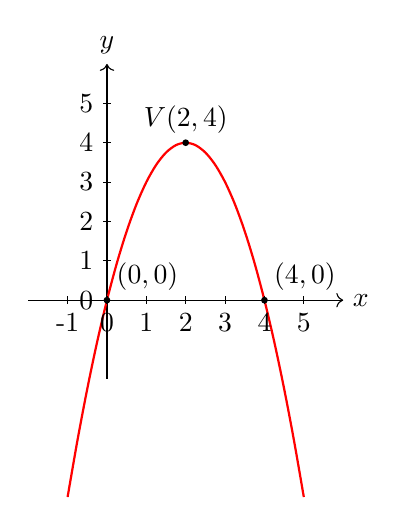
\begin{tikzpicture}[scale=0.5]
\draw[->] (-2, 0) -- (6, 0) node[right]{\(x\)};
\draw[->] (0, -2) -- (0, 6) node[above]{\(y\)};
\draw[domain=-1:5, smooth, variable=\x, red, thick] plot ({\x}, {-\x*\x + 4*\x});
\filldraw (2, 4) circle (2pt) node[above]{\(V(2, 4)\)};
\filldraw (0, 0) circle (2pt) node[above right]{\((0, 0)\)};
\filldraw (4, 0) circle (2pt) node[above right]{\((4, 0)\)};
\foreach \x in {-1,0,1,2,3,4,5}
    \draw (\x,0.1) -- (\x,-0.1) node[below] {\x};
\foreach \y in {0,1,2,3,4,5}
    \draw (0.1,\y) -- (-0.1,\y) node[left] {\y};
\end{tikzpicture}
\end{center}

a) A função possui ponto de máximo ou mínimo? Qual é esse ponto? \\
\textbf{\textcolor{blue}{Resposta:}} Possui ponto de máximo em \(V(2, 4)\), pois a concavidade é para baixo (\(a = -1 < 0\)).

b) Quais são os zeros da função? \\
\textbf{\textcolor{blue}{Resposta:}} Os zeros são \(x = 0\) e \(x = 4\).

c) Determine o valor de \(f(1)\). \\
\textbf{\textcolor{blue}{Resposta:}} Quando \(x = 1\), \(y = 3\). Portanto, \(f(1) = 3\).

d) Para que valores de \(x\) a função é positiva? \\
\textbf{\textcolor{blue}{Resposta:}} A função é positiva para \(0 < x < 4\) (a parábola está acima do eixo x).

\section*{6. Função do 2º Grau (Função Quadrática)}
Uma função do 2º grau estabelece uma relação onde a variável \(y\) depende de \(x\) de forma quadrática.

\subsection*{Definição}
Pode ser escrita na forma:
\[
f(x) = ax^{2} + bx + c
\]
onde \(a, b, c\) são constantes reais, e \(a \neq 0\).

\subsection*{Gráfico no Plano Cartesiano}
O gráfico de uma função do 2º grau é uma \textbf{parábola}. Sua concavidade depende do coeficiente \(a\):
\begin{itemize}
    \item Se \(a > 0\), a parábola tem concavidade voltada para cima (ponto de mínimo).
    \item Se \(a < 0\), a parábola tem concavidade voltada para baixo (ponto de máximo).
\end{itemize}

\subsection*{Elementos Importantes da Parábola}
\begin{itemize}
    \item \textbf{Vértice (\(V\))}: Ponto máximo ou mínimo da parábola.
    \item \textbf{Raízes (ou zeros)}: Pontos onde a parábola cruza o eixo x. São encontradas resolvendo \(ax^{2} + bx + c = 0\).
    \item \textbf{Intercepto y}: Ponto onde a parábola cruza o eixo y, dado por \(c\).
\end{itemize}

\subsection*{Atividades Resolvidas}

\textbf{Questão 1:} Identifique os coeficientes \(a\), \(b\) e \(c\) na função \(f(x) = -2x^{2} + 4x - 1\). Determine se a parábola abre para cima ou para baixo.

\textbf{\textcolor{blue}{Resolução:} }
\begin{itemize}
    \item \(a = -2\)
    \item \(b = 4\)
    \item \(c = -1\)
    \item Como \(a = -2 < 0\), a parábola tem concavidade voltada para \textbf{baixo}.
\end{itemize}

\textbf{Questão 2:} Encontre o vértice da função \(f(x) = x^{2} - 6x + 5\).

\textbf{\textcolor{blue}{Resolução:} }
Para encontrar o vértice, usamos as fórmulas:
\[
x_v = -\frac{b}{2a} = -\frac{(-6)}{2 \cdot 1} = \frac{6}{2} = 3
\]
\[
y_v = f(x_v) = f(3) = 3^{2} - 6 \cdot 3 + 5 = 9 - 18 + 5 = -4
\]
Portanto, o vértice é \(V(3, -4)\).

\textbf{Questão 3:} Resolva a equação do 2º grau \(x^{2} - 5x + 6 = 0\) e relacione as soluções com o gráfico de \(f(x) = x^{2} - 5x + 6\).

\textbf{\textcolor{blue}{Resolução:} }
Podemos resolver por fatoração ou pela fórmula de Bhaskara:
\[
x^{2} - 5x + 6 = 0 \implies (x - 2)(x - 3) = 0
\]
\[
x = 2 \quad \text{ou} \quad x = 3
\]
As soluções \(x = 2\) e \(x = 3\) são as raízes da função. Geometricamente, estes são os pontos onde a parábola cruza o eixo x: \((2, 0)\) e \((3, 0)\).

\section*{7. Aplicações e Problemas Resolvidos}

\textbf{Questão 1 (1º Grau):} Um plano de celular cobra uma taxa fixa de R\$ 30,00 mais R\$ 0,50 por minuto. Escreva a função custo \(C(x)\) e calcule o custo para 80 minutos de ligação.

\textbf{\textcolor{blue}{Resolução:} }
\[
C(x) = 0,50x + 30
\]
Para \(x = 80\) minutos:
\[
C(80) = 0,50 \cdot 80 + 30 = 40 + 30 = 70
\]
O custo para 80 minutos é de \textbf{R\$ 70,00}.

\textbf{Questão 2 (2º Grau):} O lucro \(L\) (em milhares de reais) de uma empresa é dado por \(L(x) = -x^{2} + 60x - 500\), onde \(x\) é o número de unidades vendidas (em centenas). Qual é o lucro máximo?

\textbf{\textcolor{blue}{Resolução:} }
Como \(a = -1 < 0\), a parábola tem concavidade para baixo, então o vértice representa o ponto de lucro máximo.
\[
x_v = -\frac{b}{2a} = -\frac{60}{2 \cdot (-1)} = -\frac{60}{-2} = 30
\]
\[
L_{max} = L(30) = -30^{2} + 60 \cdot 30 - 500 = -900 + 1800 - 500 = 400
\]
O lucro máximo é de \textbf{R\$ 400.000,00} (pois a função está em milhares).

\textbf{Questão 3 (Equação do 1º Grau):} Um pai tem 40 anos e seu filho tem 10 anos. Daqui a quantos anos a idade do pai será o triplo da idade do filho?

\textbf{\textcolor{blue}{Resolução:} }
Seja \(x\) o número de anos:
\[
40 + x = 3(10 + x)
\]
\[
40 + x = 30 + 3x
\]
\[
40 - 30 = 3x - x
\]
\[
10 = 2x \implies x = 5
\]
Daqui a \textbf{5 anos}, o pai terá 45 anos e o filho 15 anos (45 = 3 × 15).

\textbf{Questão 4 (Equação do 2º Grau):} Um retângulo tem comprimento 3 metros maior que a largura. Se sua área é de 40 metros quadrados, quais são suas dimensões?

\textbf{\textcolor{blue}{Resolução:} }
Seja \(x\) a largura. Então o comprimento é \(x + 3\).
\[
x(x + 3) = 40
\]
\[
x^{2} + 3x - 40 = 0
\]
Resolvendo por Bhaskara:
\[
\Delta = 3^{2} - 4 \cdot 1 \cdot (-40) = 9 + 160 = 169
\]
\[
x = \frac{-3 \pm \sqrt{169}}{2} = \frac{-3 \pm 13}{2}
\]
\[
x = \frac{-3 + 13}{2} = \frac{10}{2} = 5 \quad \text{ou} \quad x = \frac{-3 - 13}{2} = \frac{-16}{2} = -8
\]
Como largura não pode ser negativa, temos \(x = 5\) metros.
Portanto:
\begin{itemize}
    \item Largura: \(5\) m
    \item Comprimento: \(5 + 3 = 8\) m
\end{itemize}
Verificando: \(5 \times 8 = 40\) m².

\end{multicols}

\end{document}
